

\begin{frame}{Processus}

\begin{columns}
  \column{0.38\linewidth}
\begin{figure}
    \centering
    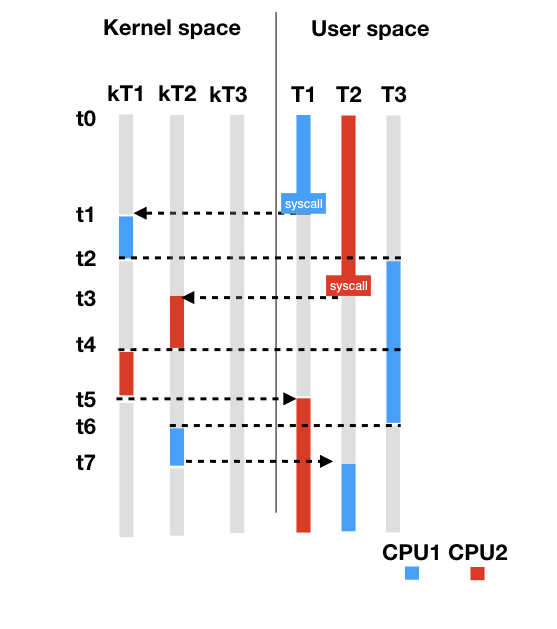
\includegraphics[width=\textwidth]{slides/images/scheduling.jpg}
\end{figure}

\column{0.58\linewidth}

\subtt{État d'un processus}

\begin{itemize}[label=$-$]
    \item Registres processeur
    \item Table des descripteurs fichiers
    \item Répertoire courant
    \item Variables d'environnement
\end{itemize}
\end{columns}

\end{frame}

\begin{frame}{\texttt{fork}}
    
    fonction Unix.fork : unit -> int

    crée un nouveau process avec le même état    
\end{frame}



\begin{frame}[fragile]{Nouvelle boucle de lecture}
\begin{lstlisting}
let minishell () =
 try
     Printf.printf "%s> %!" (Unix.getcwd ());
     while true do
       let cmd = input_line Stdlib.stdin in
       try 
         let cmd = Ast.parse cmd in
         let code = interprete cmd in
         Printf.printf "%s (%d)> %!" (Unix.getcwd ()) code
       with
       | Parser.Parsing_error err -> Parser.print_error err
       | Parser.Empty_line -> ()
     done
   with End_of_file -> ()
\end{lstlisting}
\end{frame}

\begin{frame}{\texttt{cd}}
    
\end{frame}

\begin{frame}{\texttt{fork}}

\end{frame}
